% !TeX program = pdflatex
% =============================================================
% Public Economics -- Lecture 10
% Political Economy
% Based on: Gruber, J. "Public Finance and Public Policy", Ch. 9
% =============================================================
\documentclass[11pt,aspectratio=169]{beamer}

\usetheme{metropolis}
\usepackage[utf8]{inputenc}
\usepackage[T1]{fontenc}
\usepackage{lmodern}
\usepackage{booktabs}
\usepackage{array}
\usepackage{textcomp}
\usepackage{siunitx}
\usepackage{tikz}
\usepackage{pgfplots}
\pgfplotsset{compat=1.18}
\usetikzlibrary{positioning,arrows.meta,calc}

% ----------------------------------------------------------------
% Colors: WU Vienna blue as primary accent
% ----------------------------------------------------------------
\definecolor{wublue}{HTML}{003D7C}
\definecolor{wulight}{HTML}{4F8FC4}
\definecolor{wugray}{HTML}{5C6670}
\definecolor{wured}{HTML}{B0202E}
\definecolor{wugreen}{HTML}{4C8C6B}
\definecolor{wuyellow}{HTML}{D9A441}
\setbeamercolor{palette primary}{bg=wublue,fg=white}
\setbeamercolor{frametitle}{bg=wublue,fg=white}
\setbeamercolor{progress bar}{fg=wublue,bg=wulight!30}
\setbeamercolor{alerted text}{fg=wured}

\setbeamertemplate{frame footer}{Political Economy}
\setbeamertemplate{footline}[frame number]

\title{Public Economics}
\subtitle{Lecture 10 \(\cdot\) Political Economy}
\author{Shushanik Margaryan}
\institute{WU Vienna University of Economics and Business}
\date{Winter Term}

% Source note command for footnote-style citations on data slides
\newcommand{\srcnote}[1]{{\footnotesize\color{wugray}Source: #1}}

\begin{document}

% =============================================================
\begin{frame}
  \titlepage
\end{frame}

\begin{frame}{Today's Questions}
  \begin{itemize}
    \item Public goods theory tells us \emph{how much} government should provide --- but who actually decides that amount, and how?
    \item Does majority voting reliably aggregate everyone's preferences into a sensible collective choice?
    \item If government itself is run by self-interested politicians, bureaucrats, and lobbyists, can we still trust it to fix market failures?
  \end{itemize}
  \vspace{1em}
  \begin{block}{Based on}
    Gruber, J. \emph{Public Finance and Public Policy}, Ch.\ 9 (Political Economy).
  \end{block}
\end{frame}

% =============================================================
\begin{frame}{Outline}
  \tableofcontents
\end{frame}

% =============================================================
\section{9.1 Direct Democracy}

\begin{frame}{From ``How Much'' to ``Who Decides''}
  The Samuelson rule tells us the \emph{efficient} quantity of a public good. It says nothing about \textbf{who determines} that quantity in practice.
  \begin{itemize}
    \item Real preferences for public goods are private information --- nobody has an incentive to reveal them truthfully if doing so raises their tax bill.
    \item Democracies use some form of \textbf{voting} to aggregate millions of individual preferences into one collective choice.
  \end{itemize}
  \vspace{0.4em}
  \begin{alertblock}{The central question of this lecture}
    Does the political process that decides \emph{how much} government to have itself work efficiently --- or can \emph{government failure} be just as real as market failure?
  \end{alertblock}
\end{frame}

\begin{frame}{Unanimity and the Lindahl Solution}
  \begin{block}{Lindahl pricing}
    Charge each person a personalized ``tax price'' per unit of the public good, set so that, at that price, everyone \emph{independently} demands exactly the same efficient quantity --- and unanimously agrees to it.
  \end{block}
  \vspace{0.4em}
  \textbf{Why it fails in practice:}
  \begin{itemize}
    \item Nobody has an incentive to reveal their true valuation --- understating it lowers your personalized tax price (the same preference-revelation problem from public-goods theory).
    \item Reaching genuine unanimity among millions of people is essentially impossible --- a single holdout can block everything.
  \end{itemize}
  \small In practice, societies use \textbf{majority voting} instead of unanimity --- trading away first-best efficiency for a decision rule that can actually produce a decision.
\end{frame}

% =============================================================
\section{9.2 The Median Voter Theorem}

\begin{frame}{Single-Peaked Preferences and the Median Voter Theorem}
  \begin{block}{Single-peaked preferences}
    As spending moves away from a voter's ideal point in \emph{either} direction, that voter's utility falls monotonically.
  \end{block}
  \begin{block}{Median voter theorem (Black, 1948)}
    If all voters have single-peaked preferences over a single policy dimension, majority voting selects the \textbf{median voter's} preferred outcome --- and that outcome is stable: no other option can beat it in a head-to-head majority vote.
  \end{block}
  \small This is a remarkably strong result: it doesn't matter how extreme the preferences at either tail are --- only the voter exactly in the middle determines the outcome.
\end{frame}

\begin{frame}{Diagram: The Median Voter Wins}
  \begin{center}
  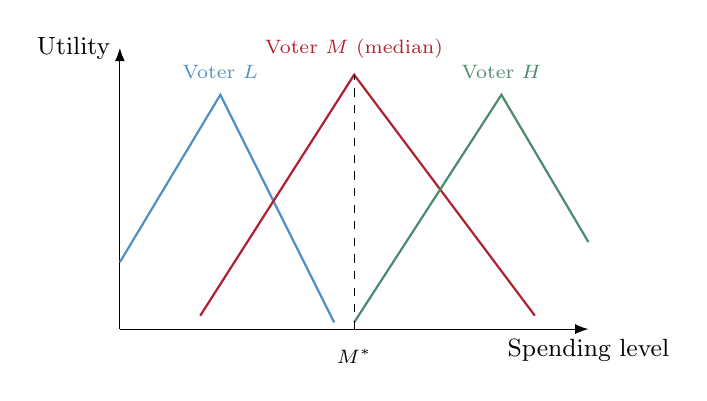
\begin{tikzpicture}[scale=0.85]
    \draw[-{Latex}] (0,0) -- (7,0) node[below, font=\small]{Spending level};
    \draw[-{Latex}] (0,0) -- (0,4.2) node[left, font=\small]{Utility};
    \draw[wulight, thick] plot coordinates {(0,1.0) (1.5,3.5) (3.2,0.1)};
    \node[above, font=\scriptsize, wulight] at (1.5,3.6) {Voter $L$};
    \draw[wured, thick] plot coordinates {(1.2,0.2) (3.5,3.8) (6.2,0.2)};
    \node[above, font=\scriptsize, wured] at (3.5,3.9) {Voter $M$ (median)};
    \draw[wugreen, thick] plot coordinates {(3.5,0.1) (5.7,3.5) (7,1.3)};
    \node[above, font=\scriptsize, wugreen] at (5.7,3.6) {Voter $H$};
    \draw[dashed] (3.5,0) -- (3.5,3.8);
    \node[below, font=\scriptsize] at (3.5,-0.15) {$M^*$};
  \end{tikzpicture}
  \end{center}
  \footnotesize With single-peaked preferences, the median voter's ideal point $M^*$ beats every other proposal in pairwise majority voting: any move toward $L$'s peak loses $M$'s and $H$'s votes; any move toward $H$'s peak loses $M$'s and $L$'s votes.
\end{frame}

\begin{frame}{When the Median Voter Theorem Breaks Down}
  The theorem requires single-peaked preferences over a \textbf{single} dimension. It can fail when:
  \begin{itemize}
    \item Choices are \textbf{multi-dimensional} (e.g., voting simultaneously on tax rates \emph{and} spending priorities) --- ``single-peaked'' may not even be well defined.
    \item Some voters have \textbf{double-peaked} preferences (e.g., someone who wants either very low or very high spending, but not a moderate compromise).
  \end{itemize}
  \begin{block}{The Condorcet paradox}
    Even with perfectly rational, transitive individual preferences, \textbf{majority voting itself can be intransitive}.
  \end{block}
\end{frame}

\begin{frame}{Illustration: The Condorcet Paradox}
  Three voters, three options, each individually rational:
  \begin{center}
  \begin{tabular}{@{}lccc@{}}
    \toprule
    & \textbf{1st choice} & \textbf{2nd choice} & \textbf{3rd choice} \\
    \midrule
    Voter 1 & A & B & C \\
    Voter 2 & B & C & A \\
    Voter 3 & C & A & B \\
    \bottomrule
  \end{tabular}
  \end{center}
  \vspace{0.5em}
  Pairwise majority votes: $A$ beats $B$ (2--1) \quad $B$ beats $C$ (2--1) \quad $C$ beats $A$ (2--1).
  \begin{alertblock}{A voting cycle}
    $A \succ B \succ C \succ A$ --- majority rule is \textbf{intransitive}, even though every individual voter is perfectly consistent. Whoever controls the voting \emph{agenda} (which pairs get voted on, in what order) can determine the winner.
  \end{alertblock}
\end{frame}

\begin{frame}{Arrow's Impossibility Theorem}
  Kenneth Arrow (1951) asked a deeper question: is there \emph{any} voting rule that avoids problems like the Condorcet paradox while satisfying basic fairness conditions?
  \begin{itemize}
    \item No dictator.
    \item Every individual preference ordering is allowed.
    \item If everyone prefers $A$ to $B$, so does society.
    \item The social ranking of $A$ vs.\ $B$ doesn't depend on preferences over some unrelated $C$.
  \end{itemize}
  \begin{alertblock}{Arrow's result}
    No voting rule can satisfy \textbf{all} of these simultaneously, once there are three or more options. There is no perfect, universally fair way to aggregate individual preferences into a social ranking.
  \end{alertblock}
\end{frame}

% =============================================================
\section{9.3 Representative Democracy}

\begin{frame}{From Direct to Representative Democracy}
  Direct voting on every policy question is impractical at national scale --- societies instead elect \textbf{representatives} who vote on their behalf.
  \begin{itemize}
    \item Representatives face their \emph{own} incentives (re-election, party loyalty, campaign funding) --- not necessarily their constituents' median preference.
    \item Representatives routinely vote on \textbf{bundles} of issues at once, opening the door to vote-trading.
  \end{itemize}
\end{frame}

\begin{frame}{Logrolling and Pork-Barrel Spending}
  \begin{block}{Logrolling}
    Trading votes across issues: ``I'll support your project if you support mine.''
  \end{block}
  \small \textbf{Example:} two projects each cost \$120 (split evenly across all districts) but benefit only \emph{one} district by \$100 each --- neither passes on its own merits. But if the two district representatives agree to support \emph{both} projects, each gets a project that benefits their own district by \$100 at a shared cost of \$120 split broadly --- and a majority coalition can form to pass both, even though neither is efficient in isolation.
  \begin{alertblock}{Legislative ``universalism''}
    When this logic generalizes across many districts, legislatures can end up approving a long list of narrowly-targeted, individually inefficient projects --- classic ``pork-barrel'' spending --- because the costs are spread thin across everyone while the benefits are concentrated.
  \end{alertblock}
\end{frame}

\begin{frame}{Special Interest Politics and Collective Action}
  \begin{block}{Olson's logic of collective action (1965)}
    A policy with \textbf{concentrated benefits} to a small group and \textbf{diffuse costs} spread across everyone else is far more likely to pass than the reverse --- even when the diffuse costs exceed the concentrated benefits.
  \end{block}
  \begin{itemize}
    \item The small group has a strong individual incentive to organize, lobby, and monitor the issue.
    \item Each individual bearing the diffuse cost has almost no incentive to fight back --- their own share of the cost is tiny (a free-rider problem, mirror image of underprovision of public goods).
  \end{itemize}
  \small This asymmetry is a standard explanation for why narrow industry protections and subsidies persist even when they plainly fail a cost-benefit test.
\end{frame}

\begin{frame}{Regulatory Capture}
  \begin{block}{Regulatory capture (Stigler, 1971)}
    Regulatory agencies, created to police an industry in the public interest, tend over time to be captured by --- and act in the interest of --- the very industry they regulate.
  \end{block}
  \begin{itemize}
    \item The regulated industry has concentrated stakes and deep expertise, and lobbies intensively.
    \item The diffuse public --- the intended beneficiary of regulation --- has little organized voice in the process.
    \item Revolving-door career patterns between regulators and industry can reinforce the alignment of interests.
  \end{itemize}
\end{frame}

% =============================================================
\section{9.4 Is Government Efficient?}

\begin{frame}{The Leviathan Model of Government}
  \begin{block}{Leviathan model (Brennan \& Buchanan, 1980)}
    Instead of a benevolent social planner maximizing welfare, treat government as a \textbf{revenue-maximizing monopolist} that expands its own size and budget as far as voters and institutions will allow.
  \end{block}
  \begin{itemize}
    \item Implication: constitutional or statutory limits on tax rates and debt aren't just red tape --- they're a deliberate check on a self-interested state.
    \item Competition \emph{between} jurisdictions (people and firms can move) is one market-like discipline on a Leviathan government --- akin to Tiebout competition.
  \end{itemize}
\end{frame}

\begin{frame}{Bureaucracy: The Niskanen Model}
  \begin{block}{Niskanen model (1971)}
    Bureaucrats are assumed to maximize their agency's \textbf{budget} (which brings prestige, staff, and influence) rather than social welfare.
  \end{block}
  \begin{itemize}
    \item A budget-maximizing bureaucracy tends to \textbf{overprovide} its service relative to the efficient level --- the mirror image of the private-sector \emph{under}provision of public goods.
    \item Because legislators often can't easily verify the agency's true cost structure, the agency can credibly claim it needs a larger budget than efficiency requires.
  \end{itemize}
  \small Not every empirical study finds bureaucratic overprovision --- but the model is a standard benchmark for thinking about principal--agent problems between voters, legislators, and the agencies that actually implement policy.
\end{frame}

\begin{frame}{Conclusion: Weighing Market Failure Against Government Failure}
  Market failure (externalities, public goods, imperfect information) is a reason government \textbf{could} improve on the market outcome --- \textbf{not} a guarantee that it \textbf{will}.
  \begin{itemize}
    \item Voting mechanisms can be manipulated, cycle, or simply fail to aggregate preferences well (median voter breakdown, Condorcet paradox, Arrow's theorem).
    \item Representatives, bureaucrats, and regulators all have their own objectives, which can diverge from social welfare (logrolling, capture, budget-maximization).
  \end{itemize}
  \begin{alertblock}{The right comparison}
    The relevant policy question is never ``markets vs.\ perfect government'' --- it is \textbf{this market failure vs.\ this specific government intervention}, warts included on both sides.
  \end{alertblock}
\end{frame}

% =============================================================
\begin{frame}{Sources}
  \tiny
  \begin{columns}[T]
    \begin{column}{0.34\textwidth}
      Arrow, K. (1951), \emph{Social Choice and Individual Values}.\\
      Black, D. (1948), \emph{JPE} 56(1).\\
      Brennan, G. \& Buchanan, J. (1980), \emph{The Power to Tax}.
    \end{column}
    \begin{column}{0.34\textwidth}
      Gruber, J., \emph{Public Finance and Public Policy}, Ch.\ 9.\\
      Niskanen, W. (1971), \emph{Bureaucracy and Representative Government}.
    \end{column}
    \begin{column}{0.34\textwidth}
      Olson, M. (1965), \emph{The Logic of Collective Action}.\\
      Stigler, G. (1971), \emph{Bell Journal of Economics}.
    \end{column}
  \end{columns}
\end{frame}

\begin{frame}[standout]
  Thank you!\\
  \vspace{0.5em}
  \small Questions and discussion
\end{frame}

\end{document}
